\cotefile{10}
\scanpage{102}
\mspage{101}

Some examples of tensor categories.

1) Let $M$ be a group. Let $\underline{C}_M$\rlap{\handwritten{\tikz[baseline=0pt,x=1em,y=1em]{\draw (0,1.25)--(.4,-.65);}}} be the category of finite-dimensional vector spaces over the field $k$, equipped with a grading of type $M$. This is a tensor category over $k$, equipped with a fibre functor over $k$, the functor ``\unsure{forgetting|forgetting|forgetting} the grading''. The associated algebraic group is the group of multiplicative type $D_k(M)$ (SGA 3 I 4.7.3). For example if $M=\underline{Z}^r$, one finds $G=\underline{G}_m^r$.

Application: let $\underline{C}$ be a tensor category over $k$ equipped with a fibre functor \inserted{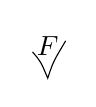
\begin{tikzpicture}[baseline=-.1ex,x=1em,y=1em]\node at (0,.9) {$F$};\draw (-.55,.7) .. controls (-.25,.35) .. (0,-.25) .. controls (.2,.35) .. (.65,1.1);\end{tikzpicture}} over $k$, hence associated with an affine group scheme $G$ over $k$\unsure{.|,} We seek all the ways of putting, for each $M\handwritten{\in}\operatorname{Ob}\underline{C}$, a grading of type $M$ on $F(V)$, functorially in $M$, and compatibly (in an obvious sense) with tensor products.Th\unsure{\rlap{l}e|e}y correspond to the $\otimes$-functors from $\underline{C}$ to $\underline{C}_M$ compatible with the fibre functors, hence to the homomorphisms from $D_k(M)$ to $G$. For example, if $M=\underline{Z}^r$, one must take the homomorphisms from $\underline{\unsure{G|E|\mathbb{G}}}_m^r$ to $G$.

In the preceding situation, one may ask when a $\otimes$-grading of type $M$ of the functor $F$ corresponds to a grading of type $M$ of the identity functor of $\underline{C}$, i.e. for every $V$, the grading of $F(V)$ comes from a grading of $V$. One finds that for this it is necessary and sufficient that the corresponding homomorphism $D_k(M)\handwritten{\longrightarrow}G$ be central. For example, if $\underline{C}$ is the category of \unsure{m\rlap{t}o\rlap{o}t\rlap{f}ives|motives} over $k$, and if one has a fiber functor $F$ on $\underline{C}$ over $k$, then one finds a canonical central homomorphism $i:\underline{G}_m\handwritten{\longrightarrow}G$. Moreover, the datum of the Tate motive (which is of rank $2$, \unsure{and|and} of ``weight'' $2$ for the natural grading) corresponds to \deleted{a} the datum of a homomorphism $j:G\handwritten{\longrightarrow}\underline{G}_m=\operatorname{Gl}(1)$. The fact that $T$ is of weight $2$ is expressed by the relation
\[
ji(\handwritten{\lambda})=\handwritten{\lambda}^{2}.
\]
